\chapter{الألكينات والألكاينات: الإضافات المحبة للإلكترونات}\label{ch:b1:electrophilic-additions}

رجّ ألكينًا مع ماء البروم البرتقالي يختفِ اللون في
ثوانٍ: إنه أقدم اختبار للرابطة الثنائية كربون--كربون. ووراءه
آلية. فإلكترونات $\pi$ في الرابطة الثنائية، المرتبطة بقوة أقل من
إلكترونات $\sigma$ والمكشوفة فوق مستوي الجزيء وتحته،
تهاجم كاشفًا فقيرًا بالإلكترونات؛ ثم يأسر الكاتيون المتكوّن
\omterm{def:b1:electronic-effects:nucleophile}{محبًا للنواة}. والخطوتان نفساهما تضيفان هاليدات الهيدروجين، والماء
والهالوجينات إلى الألكينات، وتقرّران أي كربون يتلقى أي جزء من
الكاشف، وتحددان الكيمياء الفراغية للناتج. يطوّرهما هذا الفصل،
مع القاعدة التي استخلصها كيميائي من القرن التاسع عشر من
الملاحظة \omterm{def:b1:electronic-effects:intermediates}{والكاتيون الكربوني} الذي يفسّرها.

\begin{recall}
\omterm{def:b1:electronic-effects:intermediates}{الكاتيونات الكربونية} وثباتها \omterm{def:b1:electronic-effects:curly-arrow}{والأسهم المنحنية} (\cref{ch:b1:electronic-effects})؛
ومسلّمة هاموند (\cref{prop:b1:elementary-steps:hammond})؛ والواصفان $Z$/$E$،
و\cip{R}/\cip{S}، ومركبات الميزو والخلائط الراسيمية
(\cref{ch:b1:stereochemistry-in-depth}). وقد عدّد المجلد المدرسي (الصف الثاني عشر)
إضافات الألكينات دون آلياتها.
\end{recall}

\section{الرابطة \texorpdfstring{$\pi$}{pi} محبًا للنواة}

\begin{definition}[الإضافة المحبة للإلكترونات]\label{def:b1:electrophilic-additions:electrophilic-addition}
\emph{الإضافة المحبة للإلكترونات}\index{إضافة محبة للإلكترونات} إلى
رابطة متعددة هي إضافة تكون خطوتها الأولى هجوم
إلكترونات $\pi$ على \omterm{def:b1:electronic-effects:nucleophile}{محب للإلكترونات} E: فيتكوّن كاتيون، يأسر بعد ذلك
\omterm{def:b1:electronic-effects:nucleophile}{محبًا للنواة} Nu، فينتهي E وNu على كربوني
الرابطة الثنائية السابقة.
\end{definition}

الرابطة $\pi$ هي الأضعف بين رابطتي C=C (\cref{ch:b1:lewis-resonance-vsepr})،
وإلكتروناتها بعيدة عن النوى، فوق المستوي وتحته:
فالألكينات \omterm{def:b1:electronic-effects:nucleophile}{محبات للنواة}، وتتفاعل مع الأحماض والهالوجينات وغيرها من
\omterm{def:b1:electronic-effects:nucleophile}{المحبات للإلكترونات} التي تترك الألكانات المشبعة دون مساس.

\section{إضافة هاليدات الهيدروجين: قاعدة ماركوفنيكوف}

\begin{omfigure}
\setchemfig{atom sep=2.1em}
\schemestart
\chemfig{H_3C-[:30]@{c2}CH=[@{pi},,,,]@{c1}CH_2}
\+
\chemfig{@{h}H-[@{hb}]@{br}Br}
\arrow{->}
\chemfig{H_3C-[:30]CH^{+}-[:-30]CH_3}
\+
\chemfig{Br^{-}}
\arrow{->}
\chemfig{H_3C-[:30]CH(-[2]Br)-[:-30]CH_3}
\schemestop
\chemmove{\draw[->, thick, shorten <=2pt, shorten >=2pt](pi) .. controls +(90:7mm) and +(110:7mm) .. (h);
          \draw[->, thick, shorten <=2pt, shorten >=2pt](hb) .. controls +(-90:5mm) and +(-90:5mm) .. (br);}

{\small إضافة بروميد الهيدروجين إلى البروبين. يأخذ زوج $\pi$
البروتون، على الكربون الطرفي، فيتكوّن \omterm{def:b1:electronic-effects:intermediates}{الكاتيون الكربوني} الثانوي؛ ثم يضاف إليه
أيون البروميد: 2-بروموبروبان.}
\end{omfigure}

\begin{proposition}[قاعدة ماركوفنيكوف]\label{prop:b1:electrophilic-additions:markovnikov}
في إضافة HX إلى ألكين غير متناظر، يذهب الهيدروجين إلى
كربون الرابطة الثنائية الذي يحمل أصلًا عددًا أكبر من الهيدروجينات
(\emph{قاعدة ماركوفنيكوف}\index{قاعدة ماركوفنيكوف}). وبصيغة حديثة:
يُضاف \omterm{def:b1:electronic-effects:nucleophile}{المحب للإلكترونات} بحيث يعطي \omterm{def:b1:electronic-effects:intermediates}{الكاتيون الكربوني} الأكثر ثباتًا.
\end{proposition}

\begin{proof}
انتقال البروتون هو \omterm{def:b1:elementary-steps:rds}{الخطوة المحددة للسرعة}، وهو ماص للحرارة، وينتهي إلى
\omterm{def:b1:electronic-effects:intermediates}{كاتيون كربوني}. وبمسلّمة هاموند
(\cref{prop:b1:elementary-steps:hammond}) تشبه حالته الانتقالية
\omterm{def:b1:electronic-effects:intermediates}{الكاتيون الكربوني}، فيكون للمسار المؤدي إلى الكاتيون الأكثر ثباتًا الحاجز
الأدنى، ويكون أسرع بكثير. ووضع البروتون على الكربون الذي يحمل عددًا أكبر من
الهيدروجينات يترك الشحنة على الكربون الذي يحمل عددًا أكبر من مجموعات الألكيل، وهو
الكاتيون الأكثر ثباتًا (\cref{prop:b1:electronic-effects:carbocation-order}).
\end{proof}

\begin{omfigure}
\begin{tikzpicture}
\begin{axis}[
  width=0.78\linewidth, height=5.0cm, xmin=0, xmax=10, ymin=-45, ymax=125,
  axis x line=bottom, axis y line=left, xlabel={إحداثي التفاعل},
  ylabel={الطاقة}, xtick=\empty, ytick=\empty, label style={font=\small},
  legend style={font=\scriptsize, draw=none, at={(0.5,-0.30)}, anchor=north}, legend columns=2]
\addplot[omThm, thick, dashed] table[x=x, y=E] {figdata/out/bachelor-1-energy-profiles-primary.dat};
\addplot[omDef, very thick] table[x=x, y=E] {figdata/out/bachelor-1-energy-profiles-secondary.dat};
\legend{{عبر كاتيون أولي}, {عبر كاتيون ثانوي}}
\node[font=\scriptsize, anchor=south] at (axis cs:5,103) {\ce{CH3CH2CH2+}};
\draw[omThm, densely dotted] (axis cs:5,103) -- (axis cs:5,87);
\node[font=\scriptsize, anchor=north] at (axis cs:5,43) {\ce{CH3CH+CH3}};
\node[font=\scriptsize, anchor=north west] at (axis cs:0.1,-3) {\foreignlanguage{arabic}{البروبين + \babelsublr{HBr}}};
\end{axis}
\end{tikzpicture}

{\small منحنيا طاقة تخطيطيان للإضافتين الممكنتين لبروميد الهيدروجين إلى
البروبين. يقع \omterm{def:b1:electronic-effects:intermediates}{الكاتيون الكربوني} الثانوي الأكثر ثباتًا في مستوى أدنى، وكذلك، بمسلّمة
هاموند، \omterm{def:b1:elementary-steps:energy-profile}{الحالة الانتقالية} المؤدية إليه: فيتكوّن
ناتج ماركوفنيكوف أسرع بكثير.}
\end{omfigure}

\begin{definition}[إعادة ترتيب الكاتيون الكربوني]\label{def:b1:electrophilic-additions:rearrangement}
\emph{إعادة ترتيب الكاتيون الكربوني}\index{إعادة ترتيب الكاتيون الكربوني} هي
انتقال ذرة هيدروجين أو مجموعة ألكيل، داخل \omterm{def:b1:electronic-effects:intermediates}{كاتيون كربوني}، مع
زوجها الرابط إلى الكربون الكاتيوني المجاور، فيتكوّن \omterm{def:b1:electronic-effects:intermediates}{كاتيون كربوني} أكثر
ثباتًا (انتقال 1,2).
\end{definition}

\begin{example}[انتقال مجموعة ميثيل]\label{ex:b1:electrophilic-additions:shift}
يعطي 3,3-ثنائي ميثيل بوت-1-ين وكلوريد الهيدروجين \omterm{def:b1:electronic-effects:intermediates}{كاتيونًا كربونيًا} ثانويًا
بجوار كربون رباعي؛ فتنتقل مجموعة ميثيل مع زوجها،
فيتكوّن كاتيون ثالثي. والناتج الرئيسي 2-كلورو-2,3-ثنائي ميثيل البوتان،
الذي يختلف هيكله عن هيكل الألكين؛ أما 3-كلورو-2,2-ثنائي ميثيل البوتان
فثانوي.
\end{example}

\begin{omfigure}
\setchemfig{atom sep=2em}
\schemestart
\chemfig{C(-[2]CH_3)(-[6]CH_3)(-[4]H_3C)-CH^{+}-CH_3}
\arrow{->[انتقال 1,2]}[,1.5]
\chemfig{C^{+}(-[2]CH_3)(-[4]H_3C)-CH(-[6]CH_3)-CH_3}
\arrow{->[\ce{Cl-}]}
\chemfig{C(-[2]CH_3)(-[6]Cl)(-[4]H_3C)-CH(-[6]CH_3)-CH_3}
\schemestop
\par\vspace{6pt}

{\small إعادة ترتيب الكاتيون 3,3-ثنائي ميثيل بوتان-2-يل: تنتقل مجموعة ميثيل
إلى الكربون الكاتيوني، فيتحول الكاتيون الثانوي إلى كاتيون
ثالثي، يأسره الكلوريد.}
\end{omfigure}

\section{إضافة الماء}

\begin{definition}[إماهة الألكين]\label{def:b1:electrophilic-additions:hydration}
\emph{الإماهة}\index{إماهة} في الألكين هي إضافة
الماء إليه، بحفز \omterm{def:b1:predominant-reaction:strong-acid}{حمض قوي}، فيتكوّن كحول: وهي عكس
\omterm{def:b1:alcohol-activation:dehydration}{نزع الماء} في \cref{ch:b1:alcohol-activation}.
\end{definition}

الآلية هي آلية HX مع الماء \omterm{def:b1:electronic-effects:nucleophile}{محبًا للنواة}: برتنة
(ماركوفنيكوف)، ثم أسر \omterm{def:b1:electronic-effects:intermediates}{الكاتيون الكربوني} بالماء، ثم فقد بروتون من
أيون الأوكسونيوم. فيعطي البروبين البروبان-2-أول، ويعطي 2-ميثيل البروبين
2-ميثيل البروبان-2-أول. \omterm{def:b1:electrophilic-additions:hydration}{والإماهة} \omterm{def:b1:alcohol-activation:dehydration}{ونزع الماء} هما التوازن نفسه،
\ce{C3H6 + H2O <=> C3H8O}؛ والحمض المائي المخفف ودرجة الحرارة المنخفضة يحابيان
الكحول، أما الحمض المركّز والحرارة وإزالة الألكين فتحابي
الألكين (\cref{ch:b1:extent-q-and-k}).

\section{إضافة الهالوجينات: أيونات الهالونيوم والإضافة المضادة}

\begin{definition}[أيون الهالونيوم، الإضافة المضادة والإضافة المتزامنة]\label{def:b1:electrophilic-additions:halonium}
في إضافة \ce{Br2} أو \ce{Cl2}، يهاجم زوج $\pi$ إحدى
ذرتي الهالوجين بينما يرتبط \omterm{def:b1:lewis-resonance-vsepr:lewis}{زوج حر} لتلك الذرة بالكربون الثاني:
فيتكوّن \emph{أيون هالونيوم}\index{أيون هالونيوم} حلقي ثلاثي، وتغادر
ذرة الهالوجين الأخرى على هيئة هاليد. والإضافة التي تنتهي فيها المجموعتان الجديدتان
على وجهين متقابلين للرابطة الثنائية السابقة \emph{إضافة
مضادة}\index{إضافة مضادة}؛ وعلى الوجه نفسه، \emph{إضافة
متزامنة}\index{إضافة متزامنة}.
\end{definition}

\begin{proposition}[إضافة الهالوجين مضادة]\label{prop:b1:electrophilic-additions:anti-addition}
إضافة البروم إلى ألكين \omterm{def:b1:electrophilic-additions:halonium}{إضافة مضادة}: فالبوت-2-ين-\cip{E}
يعطي 2,3-ثنائي برومو البوتان الميزو، والبوت-2-ين-\cip{Z} يعطي \omterm{def:b1:stereochemistry-in-depth:enantiomers}{الخليط
الراسيمي} من 2,3-ثنائي برومو البوتان-\cip{2R,3R} و-\cip{2S,3S}.
\end{proposition}

\begin{proof}
يجسر أيون البرومونيوم أحد وجهي الرابطة الثنائية السابقة؛ ولا يستطيع
البروميد أن يهاجم الكربون إلا من الوجه الآخر، فيفتح الحلقة كما في
SN2 مع انقلاب عند ذلك الكربون. فتنتهي ذرتا البروم على وجهين متقابلين.
ومن أجل البوت-2-ين-\cip{E}، يعطي الهجوم على أيٍّ من الكربونين الناتج نفسه، الذي
يكون فيه المركزان الفراغيان صورتين مرآويتين أحدهما للآخر: \cip{2R,3S}،
ميزو. ومن أجل البوت-2-ين-\cip{Z}، يعطي الهجوم على أحد الكربونين \cip{2R,3R}، وعلى
الآخر \cip{2S,3S}، باحتمال متساوٍ: \omterm{def:b1:stereochemistry-in-depth:enantiomers}{خليط راسيمي}. والبرهان
بالرسم هو \cref{exo:b1:electrophilic-additions:10}.
\end{proof}

\begin{omfigure}
\begin{tikzpicture}[font=\small, >={Stealth}]
  % bromonium ion from (E)-but-2-ene
  \coordinate (a) at (0,0); \coordinate (b) at (1.4,0);
  \draw[thick] (a) -- (b);
  \node[circle, fill=white, inner sep=1pt] (br) at (0.7,1.0) {\ce{Br+}};
  \draw[thick] (a) -- (br.south west) (b) -- (br.south east);
  \draw[thick] (a) -- ++(-0.8,0.35) node[left] {H};
  \draw[thick] (a) -- ++(-0.6,-0.6) node[below left] {\ce{CH3}};
  \draw[thick] (b) -- ++(0.8,0.35) node[right] {\ce{CH3}};
  \draw[thick] (b) -- ++(0.6,-0.6) node[below right] {H};
  \node (bm) at (0.7,-1.6) {\ce{Br-}};
  \draw[->, thick, omThm] (bm) to[bend left=25] (0.12,-0.12);
  \node[align=center] at (0.7,-2.4) {هجوم من الوجه المقابل للجسر};
  \draw[->, thick] (3.3,0) -- (4.4,0);
  \node[align=center] at (6.2,0) {\chemfig{C(-[:150]H_3C)(<[:210]H)(<:[2]Br)-C(<:[:30]H)(-[:-30]CH_3)(<[6]Br)}};
  \node at (6.2,-1.8) {\foreignlanguage{arabic}{ناتج مضاد: \babelsublr{2,3}-ثنائي برومو البوتان الميزو}};
\end{tikzpicture}

{\small أيون البرومونيوم المتكوّن من البوت-2-ين-\cip{E}، وفتحه
بالبروميد من الوجه المقابل (\omterm{def:b1:electrophilic-additions:halonium}{إضافة مضادة}). وللناتج مركزان
فراغيان بواصفين متعاكسين ومستوي مرآة داخلي في
\omterm{def:b1:stereochemistry-in-depth:isomers}{تشكّل} مناسب: إنه \omterm{def:b1:stereochemistry-in-depth:enantiomers}{مركب الميزو}، \cip{2R,3S}.}
\end{omfigure}

\begin{inthelab}[ماء البروم]
البروم سائل كثيف متطاير شديد السمية وأكّال. ويستعمل اختبار
عدم التشبع ماء البروم المخفف (أو محلولًا تجاريًا \omterm{def:b1:complexation:complex}{لمعقد}
للبروم) في خزانة غازات، بضع قطرات في كل مرة؛ ويدل
اختفاء اللون البرتقالي على إضافة. وفي الماء، يأسر الماء أيضًا
أيون البرومونيوم، فيتكوّن بروموهيدرين إلى جانب
ثنائي البروميد.
\end{inthelab}

\section{الألكاينات: الإضافات والأسيتيليدات}

تضيف الألكاينات HX و\ce{X2} مرتين، كل خطوة كما في الألكينات (ماركوفنيكوف
في حالة HX). وإماهتها، بحفز حمض وملح للزئبق(II)، لا تعطي
الكحول غير المشبع المتوقع بل كيتونًا: إذ يتحول الإينول فورًا
إلى مركب الكربونيل، وهي عملية تُدرس في مجلد السنة الثانية.

\begin{definition}[الألكاين الطرفي، الأسيتيليد]\label{def:b1:electrophilic-additions:acetylide}
\emph{الألكاين الطرفي}\index{ألكاين طرفي} \ce{R-C#C-H} تقع رابطته
الثلاثية في نهاية السلسلة. وتنزع \omterm{def:b1:predominant-reaction:strong-acid}{قاعدة قوية} (أميد الصوديوم)
هيدروجينه، فيتكوّن \emph{أيون الأسيتيليد}\index{أيون الأسيتيليد}
\ce{R-C#C-}، وهو \omterm{def:b1:electronic-effects:nucleophile}{محب للنواة} كربوني جيد.
\end{definition}

\begin{proposition}[حمضية الألكاينات الطرفية]\label{prop:b1:electrophilic-additions:acetylide-acidity}
الرابطة C--H في \omterm{def:b1:electrophilic-additions:acetylide}{الألكاين الطرفي} أكثر حمضيةً بكثير من روابط
الألكينات والألكانات، لكنها تبقى أقل حمضيةً بكثير من الماء: فالأسيتيليدات
تتكوّن بأيونات الأميد، لا بالهيدروكسيد، ويهدمها الماء.
\end{proposition}

\begin{proof}
في \omterm{def:b1:electrophilic-additions:acetylide}{أيون الأسيتيليد} يشغل \omterm{def:b1:lewis-resonance-vsepr:lewis}{الزوج الحر} مدارًا نصف طابعه
\textit{s} (كربون \textit{sp})، مشدودًا أقرب إلى النواة من
مدارات \omterm{def:b1:electronic-effects:intermediates}{الأنيونات الكربونية} \babelsublr{\textit{sp}$^2$} أو \babelsublr{\textit{sp}$^3$}: فهو أكثر
ثباتًا، وحمضه المرافق أقوى. لكنه يبقى قاعدة أقوى بكثير
من الهيدروكسيد، فيبرتنه الماء.
\end{proof}

يهاجم الأسيتيليد هالوجينو ألكانًا أوليًا \omterm{def:b1:nucleophilic-substitution:sn2}{بالآلية SN2} (رابطة C--C جديدة،
\ce{R-C#C-} + $\mathrm{R'Br}$) أو يُضاف إلى الكربونيل كما يُضاف \omterm{def:b1:organomagnesium:organometallic}{كاشف غرينيار}:
وهذه طريقة أخرى لبناء الهياكل الكربونية.

\begin{method}[التنبؤ بإضافة]\label{met:b1:electrophilic-additions:predict-addition}
\begin{enumerate}
  \item عيّن \omterm{def:b1:electronic-effects:nucleophile}{المحب للإلكترونات} (\ce{H+}، \ce{Br2}) \omterm{def:b1:electronic-effects:nucleophile}{والمحب للنواة}
        الذي سيليه (\ce{X-}، أو الماء، أو الهاليد).
  \item من أجل \ce{H+}: أضفه إلى الكربون الذي يعطي \omterm{def:b1:electronic-effects:intermediates}{الكاتيون الكربوني}
        الأكثر ثباتًا (ماركوفنيكوف)؛ وتحقق من احتمال انتقال 1,2.
  \item من أجل \ce{X2}: اجسر \omterm{def:b1:electrophilic-additions:halonium}{أيون الهالونيوم} وافتحه من الوجه
        المقابل (\omterm{def:b1:electrophilic-additions:halonium}{إضافة مضادة})؛ وارسم الهجومين الممكنين وقارن النواتج
        (ميزو أو راسيمي).
  \item وبوجود الماء، توقّع الكحول (أو الهالوهيدرين)
        أيضًا.
\end{enumerate}
\end{method}

\begin{history}[فلاديمير ماركوفنيكوف]
\begin{minipage}[t]{0.2\linewidth}\vspace{0pt}
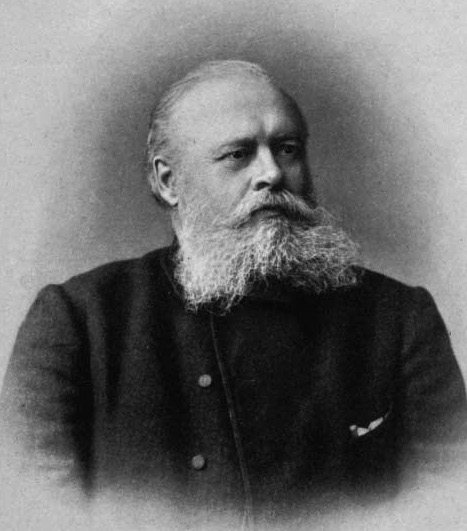
\includegraphics[width=\linewidth]{images/book2/markovnikov.jpg}
\end{minipage}\hfill
\begin{minipage}[t]{0.76\linewidth}\vspace{0pt}
صاغ فلاديمير ماركوفنيكوف قاعدته في القرن التاسع عشر، انطلاقًا من
النواتج التي لاحظها هو وغيره، قبل وجود \omterm{def:b1:electronic-effects:intermediates}{الكاتيونات الكربونية} أو \omterm{def:b1:electronic-effects:curly-arrow}{الأسهم المنحنية}
بزمن طويل: انتظامٌ في الطبيعة دُوّن قبل أن يمكن
تفسيره. وصيغتها الحديثة عبر ثبات \omterm{def:b1:electronic-effects:intermediates}{الكاتيون الكربوني} تُظهر ما
تضيفه الآلية إلى قاعدة تجريبية: فهي تقول متى ينبغي أن تخفق القاعدة.
(صورة من نعي نُشر سنة 1905، ملكية عامة،
ويكيميديا كومنز.)
\end{minipage}
\end{history}

\section{تمارين}

\begin{exercise}[$\star$]\label{exo:b1:electrophilic-additions:1}
أعطِ الناتج الرئيسي لكل من: البروبين + HCl؛ و2-ميثيل البروبين + HBr؛
و1-ميثيل الهكسين الحلقي + HBr؛ والبوت-2-اين + مكافئ واحد من HCl.
\end{exercise}

\begin{exercise}[$\star$]\label{exo:b1:electrophilic-additions:2}
اكتب نواتج البروم مع الإيثين، والهكسين الحلقي والبروبين. وسمِّ
كلًّا منها.
\end{exercise}

\begin{exercise}[$\star$]\label{exo:b1:electrophilic-additions:3}
أي كحول تعطيه \omterm{def:b1:electrophilic-additions:hydration}{الإماهة} بحفز حمضي لكل ألكين:
البروبين، و2-ميثيل البروبين، وميثيلين الهكسان الحلقي؟
\end{exercise}

\begin{exercise}[$\star$]\label{exo:b1:electrophilic-additions:4}
أي هذه المركبات يتفاعل مع أميد الصوديوم: البروباين، والبوت-2-اين،
والبروبين، والإيثانول؟ اكتب التفاعلات.
\end{exercise}

\begin{exercise}[$\star\star$]\label{exo:b1:electrophilic-additions:5}
اكتب الآلية الكاملة \omterm{def:b1:electrophilic-additions:hydration}{لإماهة} 2-ميثيل البروبين \omterm{def:b1:electronic-effects:curly-arrow}{بالأسهم
المنحنية}، وفسّر لماذا يكون التفاعل العكسي محابى في الحمض
المركّز الساخن.
\end{exercise}

\begin{exercise}[$\star\star$]\label{exo:b1:electrophilic-additions:6}
فسّر بمسلّمة هاموند لماذا يتفاعل 2-ميثيل البروبين مع HCl
أسرع بكثير من البروبين.
\end{exercise}

\begin{exercise}[$\star\star$]\label{exo:b1:electrophilic-additions:7}
يتفاعل البروم مع الهكسين الحلقي. بيّن أن الناتج هو
1,2-ثنائي برومو الهكسان الحلقي-\textit{trans}، وبيّن هل هو \omterm{def:b1:stereochemistry-in-depth:stereocentre}{كيرالي}
وهل الناتج نشط ضوئيًا.
\end{exercise}

\begin{exercise}[$\star\star$]\label{exo:b1:electrophilic-additions:8}
اقترح آلية لإضافة HCl إلى 3-ميثيل بوت-1-ين
تعطي أساسًا 2-كلورو-2-ميثيل البوتان.
\end{exercise}

\begin{exercise}[$\star\star$]\label{exo:b1:electrophilic-additions:9}
اقترح تخليقًا لهكس-2-اين من البروباين وهالوجينو ألكان،
وتخليقًا للمركب 1-فينيل بوت-2-اين-1-أول من البروباين والبنزالدهيد.
\end{exercise}

\begin{exercise}[$\star\star\star$]\label{exo:b1:electrophilic-additions:10}
برهن على الكيمياء الفراغية لإضافة البروم إلى البوت-2-ينين بالرسم:
أيون البرومونيوم، والهجوم المضاد على كل كربون، \omterm{def:b1:stereochemistry-in-depth:representations}{وتمثيل كرام}
للنواتج، والواصفات. وعُدّ \omterm{def:b1:stereochemistry-in-depth:isomers}{المتماكبات الفراغية} المتكوّنة في كل
حالة.
\end{exercise}

\begin{exercise}[$\star\star\star$]\label{exo:b1:electrophilic-additions:11}
يعطي ماء البروم مع البروبين 1-بروموبروبان-2-أول ناتجًا رئيسيًا.
فسّر الانتقائية الموضعية: لماذا يهاجم الماء الكربون الأكثر استبدالًا
في أيون البرومونيوم؟
\end{exercise}

\begin{exercise}[$\star\star\star$]\label{exo:b1:electrophilic-additions:12}
هيدروكربون \ce{C5H10} يزيل لون ماء البروم ويضيف HBr فيعطي
2-برومو-2-ميثيل البوتان؛ وتعطي إماهته 2-ميثيل البوتان-2-أول. أوجد بنيتين
ممكنتين واقترح طريقة للتمييز بينهما.
\end{exercise}

\section{مسألة: بوتينان والبروم}

\begin{problem}[{مسألة نهاية الأسبوع --- البوت-2-ينان، وآلية
البرومونيوم، وثنائيا البروميد الميزو والراسيمي، ودورانهما الضوئي
والكتلة المحصَّل عليها}]
\label{pb:b1:electrophilic-additions:1}
لدى مختبر قارورتان من البوت-2-ين، إحداهما من المتماكب \cip{Z} النقي، والأخرى من
\cip{E} النقي، ويعالج \qty{5.60}{g} من كل منهما بالبروم في
ثنائي كلورو الميثان. الكتل المولية (\unit{g/mol}): \ce{C4H8} 56.0، \ce{Br2}
159.8، \ce{C4H8Br2} 215.8.

\medskip
\noindent\textbf{الجزء الأول --- الألكينان.}
\begin{enumerate}
  \item ارسم البوت-2-ين-\cip{Z} و-\cip{E} وعلّل الواصفين.
  \item هل هما \omterm{def:b1:stereochemistry-in-depth:isomers}{متماكبان فراغيان}؟ مرآويان أم لامرآويان؟
  \item لماذا لا يتحول أحدهما إلى الآخر عند درجة حرارة الغرفة؟
  \item أيهما أكثر ثباتًا، ولماذا؟
  \item اكتب المعادلة الإجمالية لإضافة البروم.
  \item كم مركزًا فراغيًا في 2,3-ثنائي برومو البوتان؟ وكم \omterm{def:b1:stereochemistry-in-depth:isomers}{متماكبًا فراغيًا}
        على الأكثر، وكم في الواقع؟
\end{enumerate}

\medskip
\noindent\textbf{الجزء الثاني --- الآلية.}
\begin{enumerate}[resume]
  \item اكتب تكوّن أيون البرومونيوم \omterm{def:b1:electronic-effects:curly-arrow}{بالأسهم المنحنية}.
  \item لماذا يتكوّن أيون برومونيوم جسري بدل \omterm{def:b1:electronic-effects:intermediates}{كاتيون كربوني}
        مفتوح؟
  \item اكتب فتح الأيون بالبروميد.
  \item لماذا يهاجم البروميد من الوجه المقابل للجسر؟
  \item أي نوع من الإضافة ينتج؟
  \item لماذا كان المذيب ثنائي كلورو الميثان لا الماء؟
\end{enumerate}

\medskip
\noindent\textbf{الجزء الثالث --- النواتج.}
\begin{enumerate}[resume]
  \item انطلاقًا من البوت-2-ين-\cip{E}: ارسم ناتج الهجوم على C2 وأعطِ
        واصفي C2 وC3.
  \item والسؤال نفسه للهجوم على C3. قارن.
  \item بيّن أن الناتج ميزو.
  \item انطلاقًا من البوت-2-ين-\cip{Z}: ارسم الناتجين
        وواصفاتهما.
  \item بأي نسب يتكوّنان؟ سمِّ الخليط.
  \item هل \omterm{def:b1:nucleophilic-substitution:stereospecific}{التفاعل نوعي فراغيًا}؟ علّل.
\end{enumerate}

\medskip
\noindent\textbf{الجزء الرابع --- الدوران والكتلة.}
\begin{enumerate}[resume]
  \item أي دوران ضوئي يُظهره ناتج الألكين \cip{Z}؟
  \item احسب كمية كل ألكين.
  \item احسب كتلة ثنائي البروميد المتوقعة من كل منهما \omterm{def:b1:extent-q-and-k:fractional-extent}{بمردود}
        \qty{85}{\percent}.
  \item اذكر \omterm{def:b1:stereochemistry-in-depth:optical-activity}{الدوران النوعي} لثنائي البروميد المحصَّل عليه من
        البوت-2-ين-\cip{E}، والكتلة المحصَّل عليها منه.
\end{enumerate}
\end{problem}
